\documentclass[12pt]{article}
\usepackage{graphicx}
\usepackage{amsmath}
\usepackage{mathtools}
\usepackage{gensymb}

\newcommand{\mydet}[1]{\ensuremath{\begin{vmatrix}#1\end{vmatrix}}}
\providecommand{\brak}[1]{\ensuremath{\left(#1\right)}}
\providecommand{\norm}[1]{\left\lVert#1\right\rVert}
\newcommand{\solution}{\noindent \textbf{Solution: }}
\newcommand{\myvec}[1]{\ensuremath{\begin{pmatrix}#1\end{pmatrix}}}
\let\vec\mathbf

\begin{document}
\begin{center}
\textbf\large{CHAPTER-11 \\ STRAIGHT LINES}
\end{center}
\section*{Excercise 11.3}

Q3. Reduce the following equations into normal form. Find their perpendicular distances from the origin and angle between perpendicular and the positive $x$-axis.
\begin{enumerate}
	\item $x-\sqrt{3}y+8=0$ 
	\item $y-2=0$
	\item $x-y=4$
\end{enumerate}
\solution
\begin{enumerate}
\item The given equation is represented as:
	\begin{align}
	\vec{n}&=\myvec{1\\-\sqrt{3}\\}\\
	\vec{n}^\top&=\myvec{1 & -\sqrt{3}}\\
	\vec{n}^\top \vec{X}&= c\\
	\myvec{1 & -\sqrt{3}} \vec{X}&=-8\\
	\norm{\vec{n}}&=\sqrt{\vec{n}^\top.\vec{n}}\\&=\sqrt{\myvec{1&-\sqrt{3}}.\myvec{1\\-\sqrt{3}\\}}\\&=2.	
\end{align}	
	Divide the above equation(4) by 2 on both sides, we get: 
	\begin{align}
	\myvec{\frac{1}{2} & -\frac{\sqrt{3}}{2}}\vec{X}=-4
	\end{align}
	The normal form of straight line is given by:
	\begin{align}
	\vec{n}&=\myvec{\cos \theta\\\sin\theta\\}\\
	\vec{n}^\top \vec{X}&= p\\
	\myvec{\cos\theta & \sin\theta}\vec{X}&=p
	\end{align}
	By equating (8) and (11) equation, we get:
	\begin{align}
	\theta&=120^\circ\\
	p&=4
	\end{align}
	

\item The coordinates are given as
	\begin{align}
	\vec{n}&=\myvec{0\\1\\}\\
	\vec{n}^\top&=\myvec{0 & 1}\\
	\vec{n}^\top \vec{X}&= c\\
	\myvec{0 & 1} \vec{X}&=1\\
	\norm{\vec{n}}&=\sqrt{\vec{n}^\top.\vec{n}}\\&=\sqrt{\myvec{0&1}.\myvec{0\\1\\}}\\&=1.	
\end{align}	
	Divide the above equation(17) by 1 on both sides, we get: 
	\begin{align}
	\myvec{0 & 1}\vec{X}=1
	\end{align}
	The normal form of straight line is given by:
	\begin{align}
	\vec{n}&=\myvec{\cos \theta\\\sin\theta\\}\\
	\vec{n}^\top \vec{X}&= p\\
	\myvec{\cos\theta & \sin\theta}\vec{X}&=p
	\end{align}
	By equating (21) and (24) equations, we get:
	\begin{align}
	\theta&=90^\circ\\
	p&=1
	\end{align}

	
\item The coordinates are given as
	\begin{align}
	\vec{n}&=\myvec{1\\-1\\}\\
	\vec{n}^\top&=\myvec{1 & -1}\\
	\vec{n}^\top \vec{X}&= c\\
	\myvec{1 & -1} \vec{X}&=4\\
	\norm{\vec{n}}&=\sqrt{\vec{n}^\top.\vec{n}}\\&=\sqrt{\myvec{1&-1}.\myvec{1\\-1\\}}\\&=\sqrt{2}.	
\end{align}	
	Divide the above equation(30) by $\sqrt{2}$ on both sides, we get: 
	\begin{align}
	\myvec{\frac{1}{\sqrt{2}} & -\frac{1}{\sqrt{2}}}\vec{X}=2\sqrt{2}
	\end{align}
	The normal form of straight line is given by:
	\begin{align}
	\vec{n}&=\myvec{\cos \theta\\\sin\theta\\}\\
	\vec{n}^\top \vec{X}&= p\\
	\myvec{\cos\theta & \sin\theta}\vec{X}&=p
	\end{align}
	By equating (34) and (37) equations, we get:
	\begin{align}
	\theta&=45^\circ\\
	p&=2\sqrt{2}
	\end{align}

\begin{figure}[!h]
	\begin{center} 
	    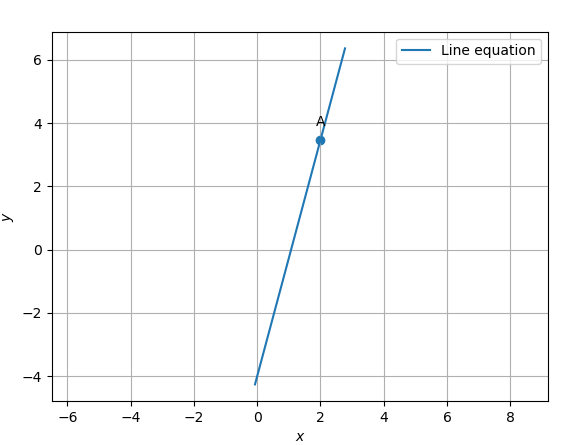
\includegraphics[width=\columnwidth]{./figs/line.png}
	\end{center}
\caption{}
\label{fig:Fig}
\end{figure}
\end{enumerate}
\end{document}